\documentclass[sigplan,screen]{acmart}

%%
%% \BibTeX command to typeset BibTeX logo in the docs
\AtBeginDocument{%
	\providecommand\BibTeX{{%
Bib\TeX}}}

\usepackage{emoji}
\usepackage{csquotes}

% \setemojifont{Apple Color Emoji}

\begin{document}

\title{GNU, Free software and Stallman's dedication}

\author{Stan Ioan-Victor 832}
\email{ioan.victor.stan@stud.ubbcluj.ro}

\begin{teaserfigure}
	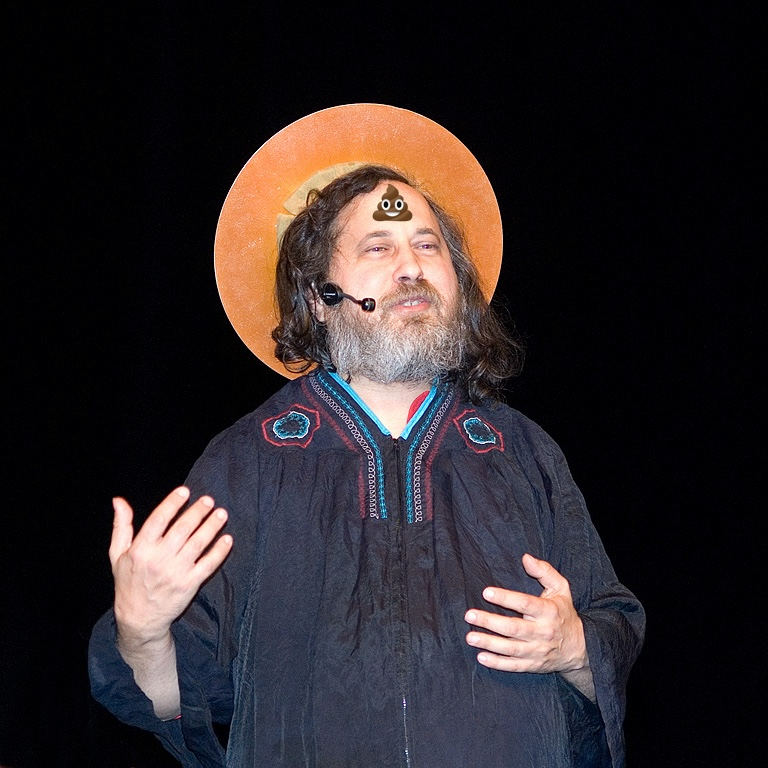
\includegraphics[width=200px]{pics/jesus-stallman.jpg}
	\centering
	\caption{RMS in his divine prime}
	\Description{Enjoying the baseball game from the third-base
	seats. Ichiro Suzuki preparing to bat.}
	\label{fig:teaser}
\end{teaserfigure}

%% This command processes the author and affiliation and title
%% information and builds the first part of the formatted document.
\maketitle

One of (I feel like) most important key aspects that often goes overlooked in today's "SIGN UP HERE, SUBSCRIBE THERE, ACCEPT MY COOKIESS PlsPLSPLPS" age is privacy and freedom of your personal data or just having technology DO WHAT YOU NEED/WANT IT TO, where now \href{https://www.youtube.com/watch?v=MPyJBJTHyO0}{Facebook requires 1384 hoola hoops}\cite{tantacrul} through which you need to jump just to exercise your right to be forgotten, and where \href{https://www.youtube.com/watch?v=LZzubS1ILTs}{Microsoft shoves ads down your throat}\cite{jakey} when you use their bloated Windows "file search" \textbf{dis-service}\cite{BarraDRM} that forces your prompt through Bing. It's such a shame because these computing things are amazing, they just got handcuffs on them.

But this guy, \textbf{up above} was concerned we might come to this before there even was any code highlighting.

\textbf{Richard Matthew Stallman} (rms) was right in a way, since his cautionary tale all the way back from '97: \href{https://www.gnu.org/philosophy/right-to-read.html}{The Right to Read}\cite{Stallman1997TheRT} has become kind of true over the past years, when services that you technically don't own get re-branded as "products"\cite{product}, but they could rug-pull you at any moment, everything from film\cite{jellyfin}, to of course, as the previous citations pointed out, literature and education.

So how did we get here, and when did my mans realize a change is needed?

\section{That damn symbolics.com}
In the early 80's, Stallman was working on his lil version of the Lisp interpreter, when software conglomerate \href{https://symbolics.com}{symbolics} asked if they could use it for a bit (will give it back unworn promise ongong fr \emoji{crossed-fingers}). You see, Symbolics is a manufacturer of exactly \ldots \textbf{ Lisp machines}, which are exactly what they sound like.

What's important about them is: they are, believe it or not, actually so OG, they were the veryy first \textbf{domain name} ever registered on the internet in 1985. Wayy before ICANN was even a thing and they had to shake hands with "the National Science Foundation (NSF)". ICANN only came out in '95. \cite{national-science-foundation}

Now since Stallman accepted to give them the interpreter via a \textbf{public domain} lisence, they had no qualms about modifying it and keeping it in-house. He then tried to ask for those mods back but he never got them.

His grudge was so intense after that incident that he decided to start the

\section{Free software movement}
In '83 (rms) launched an OS that would be like Unix, in the sense of its impact and user experience, but not in the sense of how locked-down it was to modifications and its proprietary nature, Unix being owned by AT\&T primarily. He came up with the genious (\verb|\s|) recursive acrnonym of \textbf{G}NU's not Unix. Cuz it wasn't\ldots. “GNU” was too damn good they even named an asteriod after it. \cite{gnu-asteriod} He basically set out to “free” Unix.

The philosophy behind “free” is the main point of contention for a lot of people learning about the free software movement.

This doesn't mean there can't be ANY restrictions when distributing modified versions.

In fact, even the copy of the original, free \verb|sample-sigplan.tex| file distributed by ACM that I used for this double-column format had the requirement of

//TODO scrie despre blalblal gotta boo gyygyeg

\begin{displayquote}
	"
	Any modified versions of this file must be renamed
 with new filenames distinct from \verb|sample-sigplan.tex|
	"
\end{displayquote}
and
\begin{displayquote}
	"
	This generated file may be distributed as long as the
 original source files, as listed above, are part of the
 same distribution.
	"
\end{displayquote}

What the FSF has to say about this is
\begin{displayquote}
	"
	This sort of requirement is acceptable only if there's a suitable aliasing facility that allows you to specify the original program's name as an alias for the modified version.
	"
\end{displayquote}
And I mean … I only ever had to change the name of \textbf{this} file and everything else just snapped into place.

% ca na, sa ma lase sa compilez
\nocite{*}

\bibliographystyle{ACM-Reference-Format}
\bibliography{biblio}

%% If your work has an appendix, this is the place to put it.
% \appendix

\end{document}
\endinput
